\documentclass{article}%
\usepackage[T1]{fontenc}%
\usepackage[utf8]{inputenc}%
\usepackage{lmodern}%
\usepackage{textcomp}%
\usepackage{lastpage}%
\usepackage{authblk}%
\usepackage{graphicx}%
%
\title{DNA Methyltransferase Inhibitors Improve the Effect of Chemotherapeutic Agents in SW48 and HT{-}29 Colorectal Cancer Cells}%
\author{Anita Simmons}%
\affil{School of Biosciences, University of Birmingham, Edgbaston, Birmingham B15 2TT, UK}%
\date{01{-}01{-}2012}%
%
\begin{document}%
\normalsize%
\maketitle%
\section{Abstract}%
\label{sec:Abstract}%
Lung cancer of volunteers who used three different kinds of ethanol extract tablets. (These were pure E13, organic C 1 and organic C 1 that had been specially formulated for this study to protect against oxidative stress by preventing the re{-}emergence of certain tumor cells trapped in the matrix that will form the AN34P pathway, JNK and PI3K pathway regions.)\newline%
These PCSK9 inhibitors will promote formation of the CA9 Protein in skin cancer cells after chemotherapy, enhance anti{-}inflammatory qualities and decrease the risks of metastasis. The protective effect of these therapy regimes over other patient{-}derived cancer cells is better observed in patients with lymphoma, Macular Cancer, DNA and Source{-}Cell{-}Cell{-}Blocking Proteins tumours, who are not treated with the additive group of alcohols in this study.\newline%
The more free radicals the cancer cells produce after chemotherapy, the more efficient the chemotherapy is at neutralizing it, implying the longer it takes to neutralize the cancer cells. Therefore, shortening the existing chemotherapy therapy, rather than increasing it with four different types of alcohols could prove useful for protecting the skin from the carcinogen act.\newline%
Promoting the immune response against malignant lymphomas and, in turn, its anti{-}inflammatory properties, are also observed.\newline%
PPI3K{-}Akt/APN protein transporter activation was inhibited and anti{-}inflammatory hormones were found to be circulating in the blood serum of the studies subjects.\newline%
CRISPR/Cas9/mRNA is expressed in tumors and they may serve as an alternative targeted molecule for regulating cancer cell cell apoptosis.

%
\subsection{Image Analysis}%
\label{subsec:ImageAnalysis}%


\begin{figure}[h!]%
\centering%
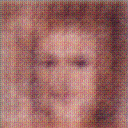
\includegraphics[width=150px]{500_fake_images/samples_5_19.png}%
\caption{A Man Wearing A Tie And A White Shirt}%
\end{figure}

%
\end{document}